\begin{evenBlock}{Touchdown Passing}
\begin{minipage}[t]{\linewidth}
    \begin{minipage}{.3\linewidth} % Left column and width
        \centering
        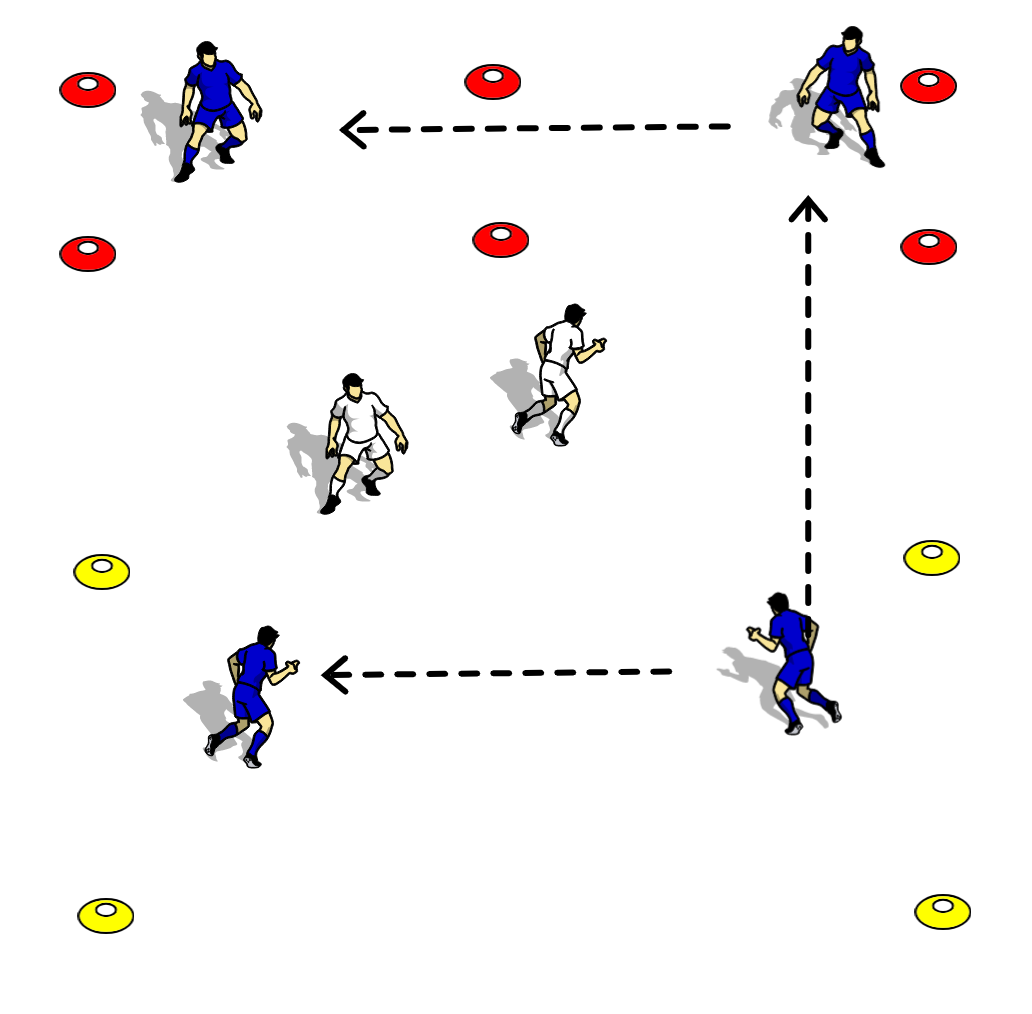
\includegraphics[width=.7\textwidth]{../img/Trimmed/TouchDownPassing}
    \end{minipage}
    \hspace{0.05\linewidth}
    \begin{minipage}{.6\linewidth} % Left column and width
        \textbf{Drill Description:}
        This drill requires 3 pairs of boys.  Pair one are receivers in the end zone.  The second pair are defenders and the last pair are the `quarterbacks' (passers).  The ball starts in the end zone and is passed out to an open passer.  That passer then passes to their partner or back into the touchdown zone. The defenders try and intercept the pass, if they do it successfully, they become the passers and the passers become the defenders.  If the end zone players (receivers pass the ball out of bounds they become the defenders and the defense becomes the receivers.)
        %\begin{enumerate}
        %    \setlength{\itemsep}{0pt}
        %    \setlength{\parskip}{0pt}
        %    \setlength{\parsep}{0pt}
        %    \item All players stand `open' so they can see the other two players.
        %    \item The ball should be passed on one direction to start (to the left is more natural for a right footed player).
        %    \item The player receiving the ball should move his body so he receives the ball on his left foot then passes it to the next player using his right.  However the pass should wait until the 3 player is in position.
        %    \item  Player 3 (P3) was at a corner nearest the ball, however once the ball was passed, P3 needs to move to the other corner so they are again at a corner adjacent to the player with the ball.
        %    \item After 5 rounds around the box, switch directions.  Pass to the right using the left foot, trap with the right.
        %    \item After 5 additional rounds allow the player to switch directions at will, but any two adjacent players can't pass the ball back and forth more than 3 times.
        %\end{enumerate}
    \end{minipage}
\end{minipage}
\raggedright
    \textbf{Coaching Points:}
    \begin{itemize}
        \setlength{\itemsep}{0pt}
        \setlength{\parskip}{0pt}
        \setlength{\parsep}{0pt}
        \item Explain the first touch with the correct foot is the most important part.
        \item The touch should place the ball one step away from the player so they can step into and make a strong pass.
        \item The goal is to use two touches, not 1 and not 3.
    \end{itemize}

\end{evenBlock}